\documentclass{article}
\usepackage{graphicx}
\usepackage[table,xcdraw]{xcolor}
\usepackage{tabularx}
\usepackage{adjustbox}
\usepackage{subcaption}
\usepackage{mathtools}
\usepackage{amsmath}
\usepackage[thinc]{esdiff}
\usepackage{lipsum}  
\usepackage{float}
\usepackage{lmodern,adjustbox,booktabs,multirow}
\usepackage{titlesec}

\usepackage[english]{babel}

\usepackage[letterpaper,top=2cm,bottom=2cm,left=3cm,right=3cm,marginparwidth=1.75cm]{geometry}

\titleformat{\section}
  {\normalfont\normalsize\bfseries}{Unit \thesection.}{1em}{}

\usepackage{amsmath}
\DeclareMathOperator{\arcsec}{arcsec}
\DeclareMathOperator{\arccot}{arccot}
\DeclareMathOperator{\arccsc}{arccsc}
\newcommand{\letv}[1]{\text{let }#1 = }
\newcommand{\intbar}{\biggr\rvert}
\usepackage{amssymb}
\usepackage[colorlinks=true, allcolors=blue]{hyperref}

\title{AP Calculus AB Notes}
\author{Daniel Hart}
\date{2024 - 2025}

\begin{document}

\maketitle

\section{Limits}
\begin{itemize}
    \item A Limit is the intended height of a graph, as x gets very close to a value.
    \item A Removable discontinuity is a hole discontinuity, whilst a Non-removable discontinuity are jumps and infinite discontinuities
    \item When solving for limits plug in c for x and always write $\frac{0}{0}$ when the limit after you plug x in is $\frac{0}{0}$
    \[\text{To prove }\lim_{x\to c}f(x)\text{ by Squeeze theorem:}\]
    \begin{enumerate}
        \item Prove that:
            $f(x)\text{ is between functions }g(x)\text{ and }h(x)\text{ this is written as }g(x) \leq f(x) \leq h(x)$
        \item Prove that: \[
            \lim_{x\to c}g(x) = \lim_{x\to c}h(x)
        \]
        \item Write that: \[\therefore\text{ By Squeeze Theorem } \lim_{x\to c}f(x) =\text{ the result of the limits got in the second step}\]
    \end{enumerate}
    
    \begin{figure}[H]
        \centering
        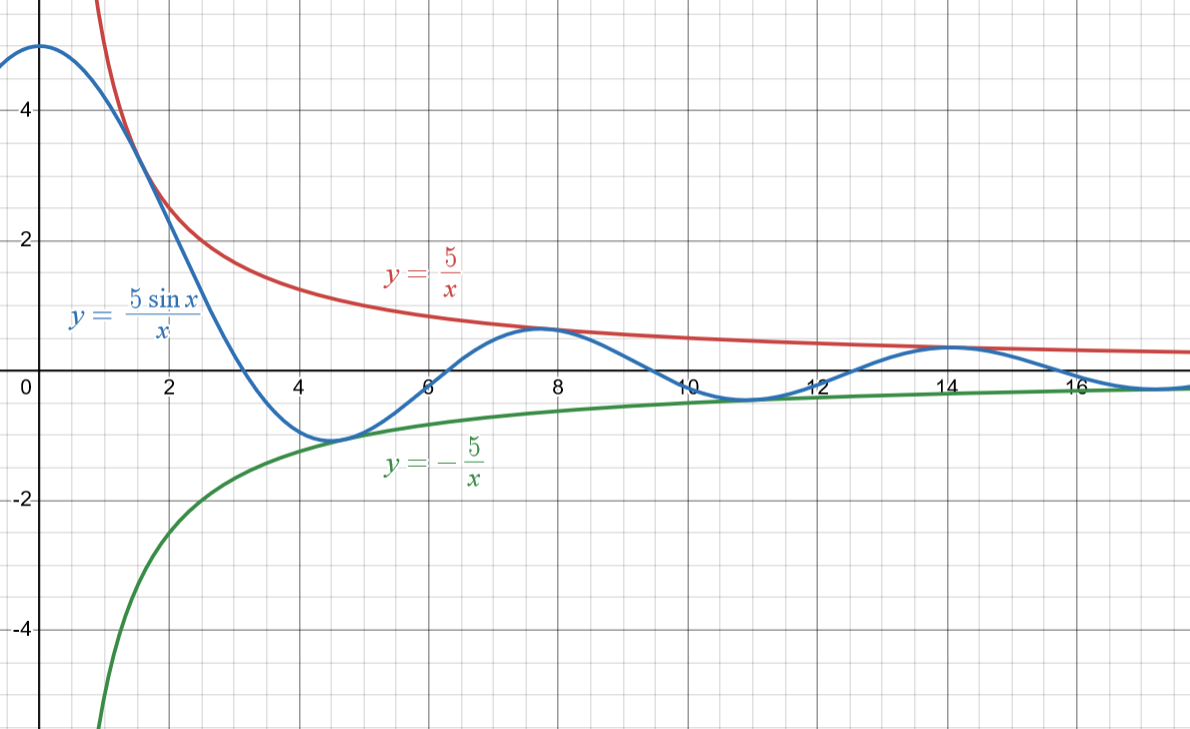
\includegraphics[width=0.5\linewidth]{images/Squeeze Theorem Graph.png}
        \caption{Squeeze Theorem Graph}
    \end{figure}
    
    \item When proving a value is in a function by IVT (Intermediate Value Theorem)
    \begin{enumerate}
        \item Prove that: $f(x)$ is continuous over a range such as $[a,b]$
        \item Write each value $f(a)=c$ and $f(b)=d$
        \item Prove that: $f(a) < \text{value} < f(b)$
        \item Write that $\therefore$ by IVT $\exists k \text{ s.t. } f(k) =$ value
    \end{enumerate}
\end{itemize}

\newpage
\section{Derivatives}
\begin{itemize}
    \item Tangent lines are lines that touch a curve at one point
    \item The definitions of a Derivative are
    \begin{align*}
        f'(x) &= \lim_{h\to 0} \frac{f(x+h) - f(x)}{h} \\
        f'(x) &= \lim_{h\to 0} \frac{f(x+h) - f(x-h)}{2h} \\
        f'(a) &= \lim_{x\to a} \frac{f(x) - f(a)}{x-a}
    \end{align*}
    
    \item A derivative of a function $f(x)$ can be written as $f'(x)$, $\diff{}{x} f(x)$, or $\diff{f}{x}$
    \item If written as an equation ($y=$...) then the derivative can be written as $y'$ or $\diff{y}{x}$
    \item To find the tangent lines of a function
    \begin{enumerate}
        \item Find f'(x)
        \item Write in point slope form: $y - y_1 = f'(x_1)(x - x_1)$
    \end{enumerate}
    \item To find the normal lines of a function
    \begin{enumerate}
        \item Find f'(x) or a tangent line
        \item Write in point slope form: $y - y_1 = -\frac{1}{f'(x_1)}(x - x_1)$
    \end{enumerate}
    \item To find a horizontal tangent line solve for x when $f'(x) = 0$
    \item A function is differentiable when differentiable at every point
    \item A function is differentiable at a point when the limit exists 
    \item Derivative Rules
    \begin{itemize}
        \item Derivative of a Constant function: if $c$ is a constant, then $\diff{}{x} c = 0$
        \item Power Rule: $\diff{}{x} ax^b = abx^{(b-1)}$
        \item Product Rule: $\diff{}{x} uv = uv' + vu'$
        \item Quotient Rule: $\diff{}{x} \frac{u}{v} = \frac{vu' - uv'}{v^2}$
        \item Log Rule: $\diff{}{x} \log_bx = \frac{1}{x\ln b}$
        \item Exponential Rule: $\diff{}{x} a^x = a^x\ln a$
        \item Trig Derivatives
        \begin{equation*}
            \begin{aligned}[c]
            \diff{}{x} \sin x &= \cos x \\
            \diff{}{x} \sec x &= \sec x \tan x \\
            \diff{}{x} \tan x &= \sec^2 x
            \end{aligned}
            \qquad
            \begin{aligned}[c]
            \diff{}{x} \cos x &= -\sin x \\
            \diff{}{x} \csc x &= -\csc x \cot x \\
            \diff{}{x} \cot x &= \csc^2 x
            \end{aligned}
        \end{equation*}
    \end{itemize}
\end{itemize}

\newpage
\section{Composite, Inverse, and Implicit Derivatives}
\begin{itemize}
    \item Chain rule says $(f\circ g)'(x) = f'(g(x))g'(x)$
    \item To find the derivative using implicit differentiation:
    \begin{enumerate}
        \item Differentiate both sides in Leibniz notation and remember that y is a function of x so you need to apply the chain rule
        \item If necessary distribute into separate terms
        \item Move all terms with $\diff{y}{x}$ to one side of the equation and all other terms to the other side
    \end{enumerate}
    \item The derivative of an inverse function is $\frac{1}{f'(f^{-1}(x))}$
    \item Inverse Trig Derivatives
        \begin{equation*}
            \begin{aligned}[c]
            \diff{}{x} \arcsin x &= \frac{1}{\sqrt{1-x^2}} \\
            \diff{}{x} \arctan x &= \frac{1}{1+x^2} \\
            \diff{}{x} \arcsec x &= \frac{1}{|x|\sqrt{x^2-1}}
            \end{aligned}
            \qquad
            \begin{aligned}[c]
            \diff{}{x} \arccos x &= \frac{-1}{\sqrt{1-x^2}} \\
            \diff{}{x} \arccot x &= \frac{-1}{1+x^2} \\
            \diff{}{x} \arccsc x &= \frac{-1}{|x|\sqrt{x^2-1}}
            \end{aligned}
        \end{equation*}
\end{itemize}

\newpage
\section{Analytical Applications of differentiation}
\begin{itemize}
    \item A critical point on a graph is when $f'=0$ but not including an endpoint
    \item To find the Absolute max and min plug in for both endpoints, and all critical points
    \item To find local minimums and maximums either graph $f'$'s sign or find the sign of $f''$
    \item To find a slope on a function interval by MVT (Mean Value Theorem):
    \begin{enumerate}
        \item Prove $f$ is continuous $[a,b]$
        \item Prove $f$ is differentiable $(a,b)$
        \item Find the average rate of change of the interval $[a,b]$:
        \[
            \frac{f(b)-f(a)}{b-a}
        \]
        \item Write $\therefore$ by MVT $\exists c\in(a,b)$ s.t. $f'(c) =$ the average rate of change
    \end{enumerate}

    \begin{figure}[H]
        \centering
        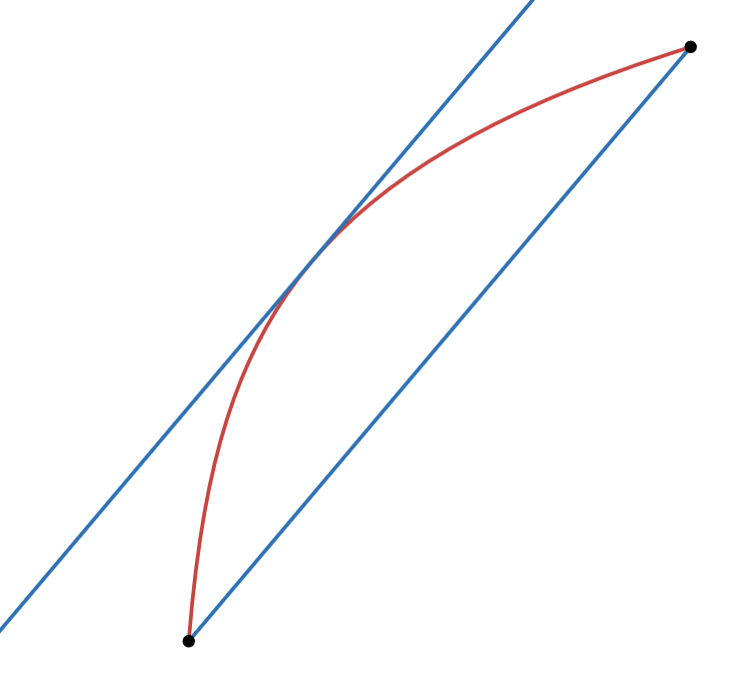
\includegraphics[width=0.5\linewidth]{images/MVT graph.png}
        \caption{MVT graph}
    \end{figure}
\end{itemize}

\newpage
\section{Contextual Applications of Differentiations}
\begin{itemize}
    \item Remember Geometric Equations for volume and surface area for 3D shapes
    \item And area and perimeter for 2D shapes see Figure \ref{fig:geometricEquations}
    \begin{figure}[h]
        \centering
        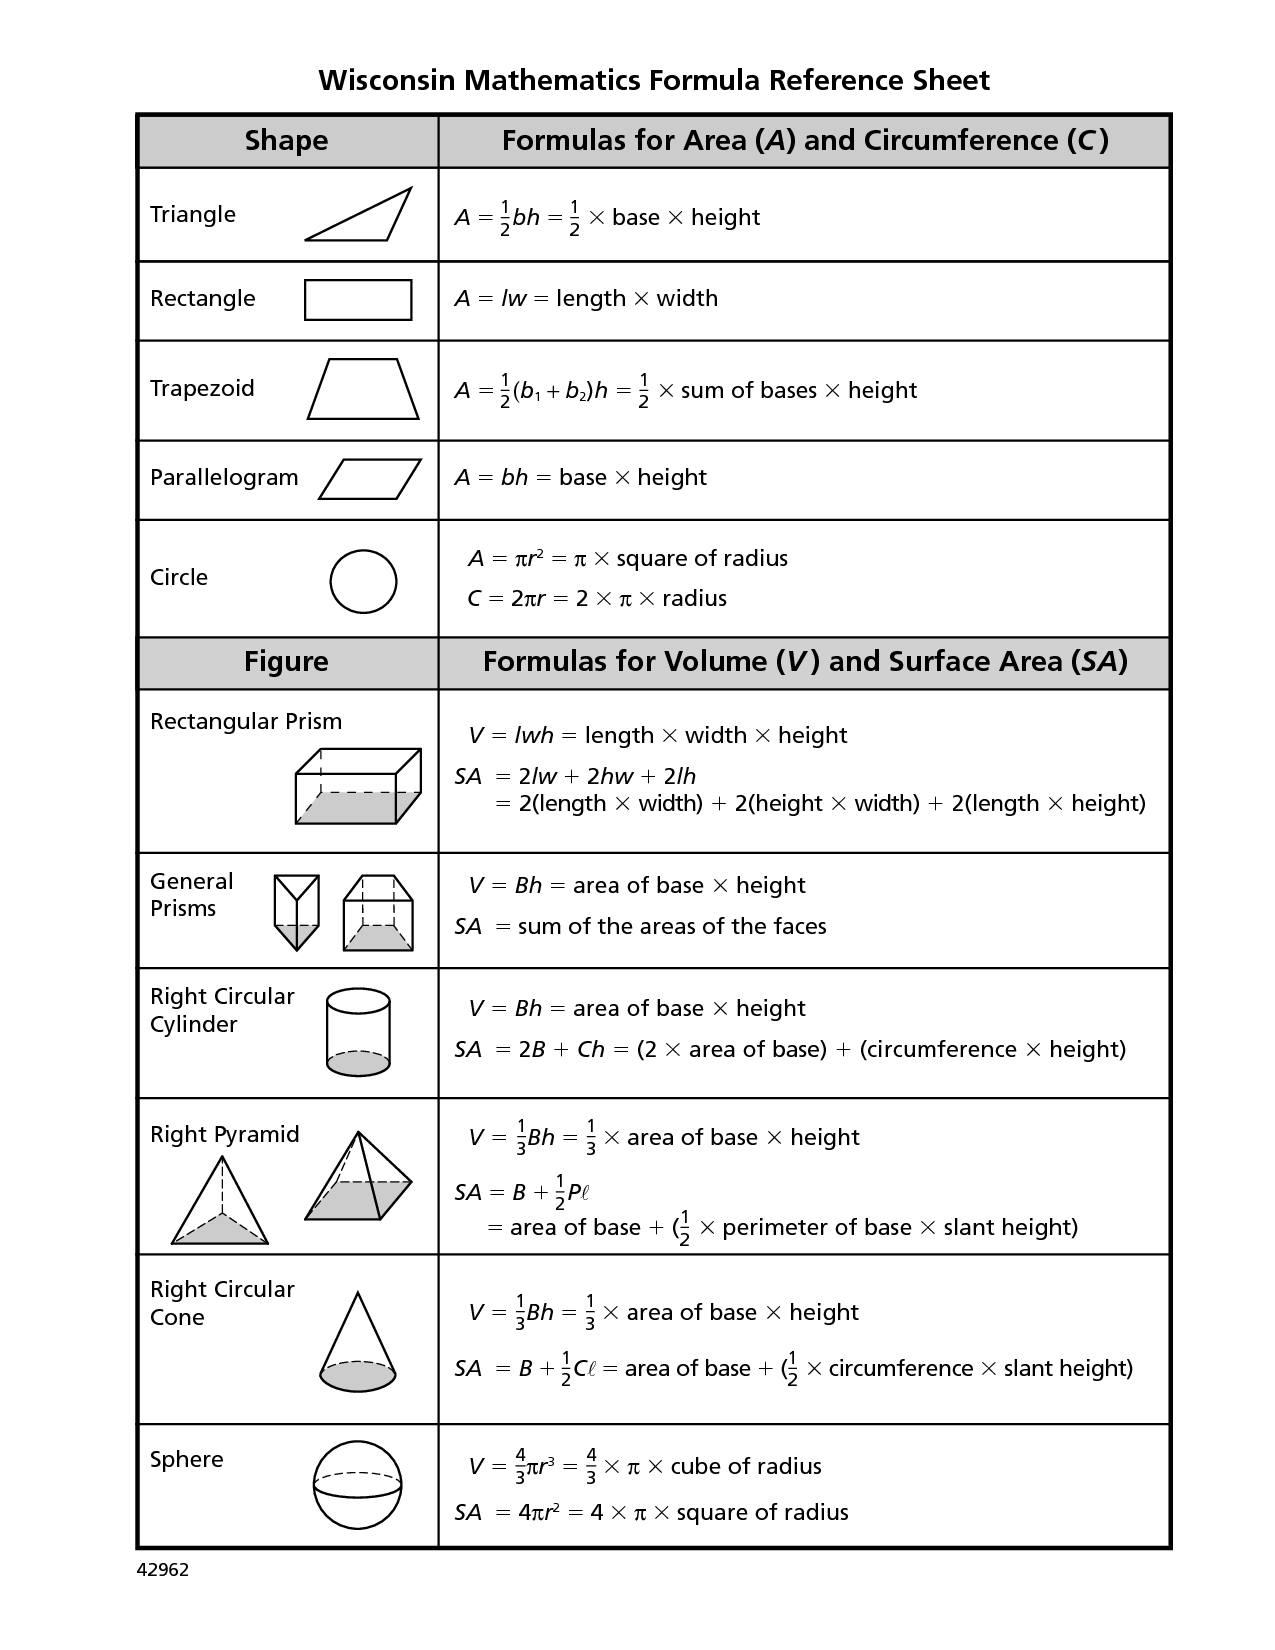
\includegraphics[width=0.5\linewidth]{images/Geometric Equations.png}
        \caption{Geometric Equations}
        \label{fig:geometricEquations}
    \end{figure}
    \item To solve for related rates:
    \begin{enumerate}
        \item Draw or look at a drawing of the shape
        \item Write what you know
        \item Write an equation relating the variables
        \item Differentiate both sides
        \item Plug in what you know
        \item Solve for wanted rate
    \end{enumerate}
    \item Example: The volume of a cube see Figure \ref{fig:cube}, is increasing at a rate of 20 cm$^3$/sec. How fast is the surface area of the cube increasing at the instant when each edge of the cube is 5 cm long?
    \begin{enumerate}
        \item \begin{figure}[h]
            \centering
            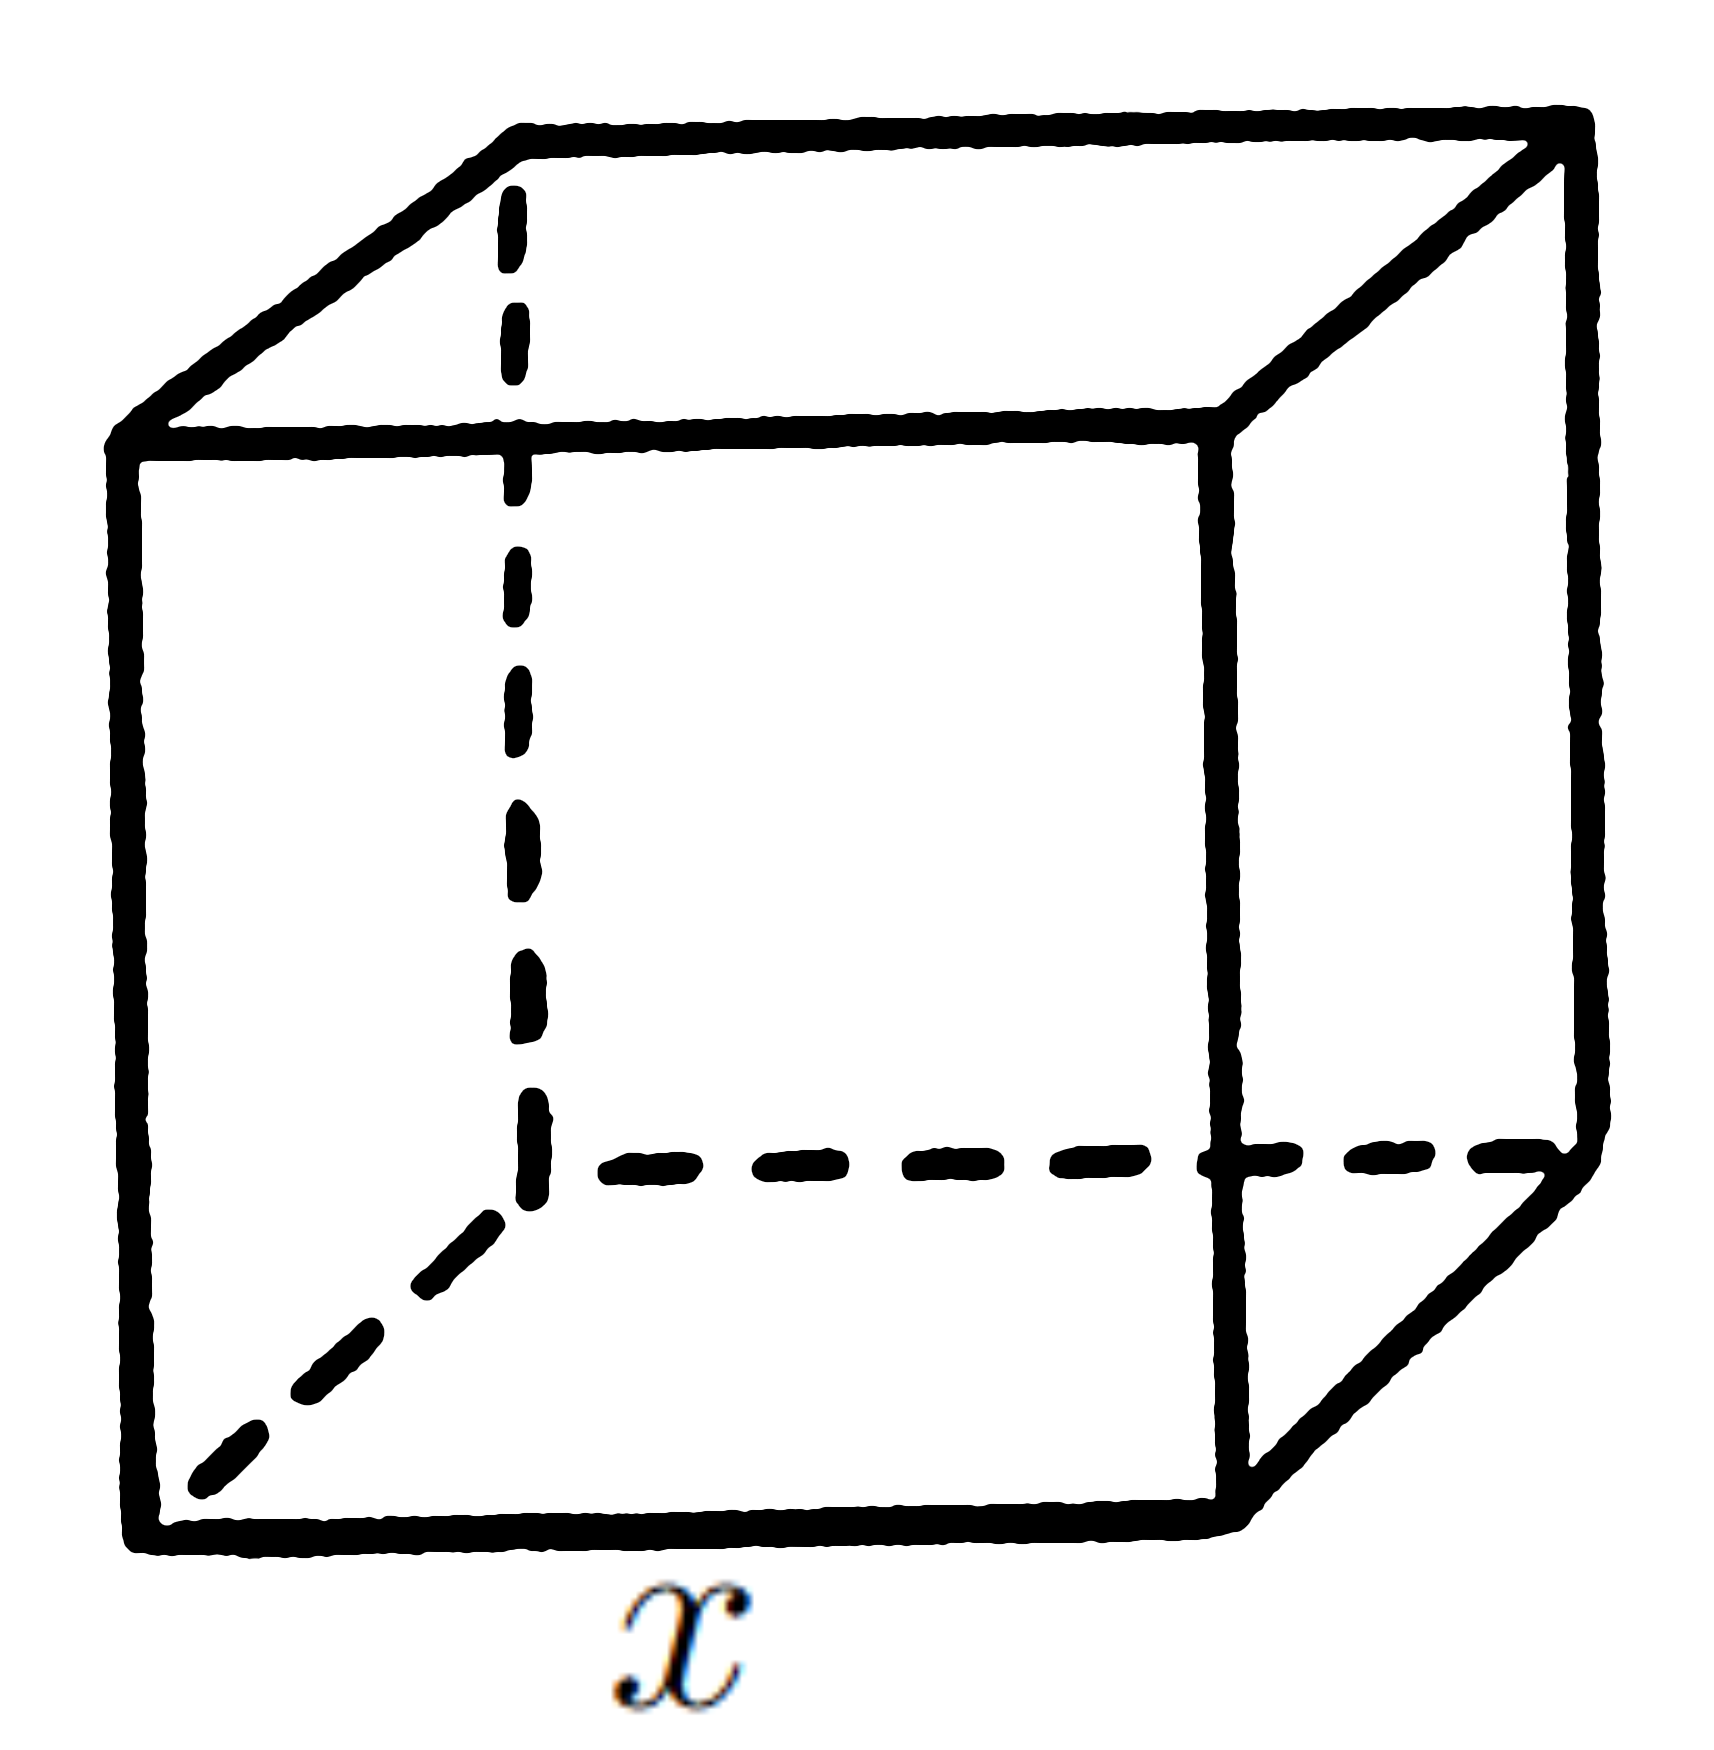
\includegraphics[width=.2\linewidth]{images/Cube.png}
            \caption{Cube Diagram}
            \label{fig:cube}
        \end{figure}
        \item Know: $\diff{V}{t} = 20 \frac{\text{cm}^3}{\text{sec}}$
        \item Find $\diff{SA}{t}$ when $x=5$
        \item $V = x^3$
        \item $\diff{V}{t} = 3x^2 \diff{x}{t}$
        \item $20 = 3(25) \diff{x}{t}$ \\
        $\implies\diff{x}{t} = \frac{4}{15} \frac{\text{cm}}{\text{sec}}$
        \item[4.] $SA = 6x^2$
        \item[5.] $\diff{SA}{t} = 12x\diff{x}{t}$
        \item[6.] $\diff{SA}{t} = 12(5)(\frac{4}{15}) = \boxed{16 \frac{\text{cm}^2}{\text{sec}}}$
    \end{enumerate}
    \item Example: In Figure \ref{fig:baseballSquare}, a baseball field is a square of side 90 feet. If a runner on second base (II) starts running toward third base (III) at a rate of 20 ft/sec, how fast is his distance from home plate (H) changing when he is 30 ft from third base (III)?
    \begin{enumerate}
        \item \begin{figure}[h]
            \centering
            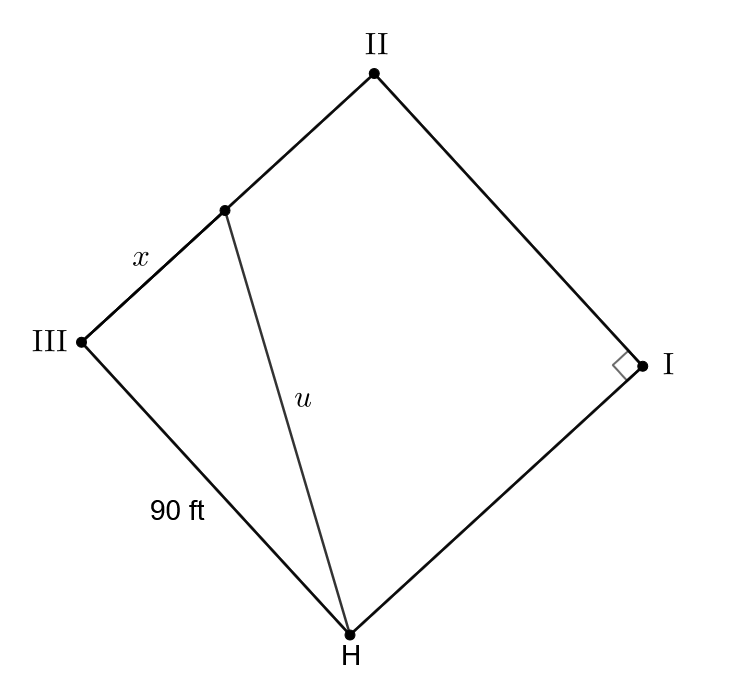
\includegraphics[width=.4\linewidth]{images/Baseball Square.png}
            \caption{Baseball Square}
            \label{fig:baseballSquare}
        \end{figure}
        \item Know $\diff{x}{t} = 20 \frac{\text{ft}}{\text{sec}}$
        \item Find $\diff{u}{t}$ when $x = 30$
        \item $x^2 + 90^2 = u^2$
        \item[4.1.] $u = \sqrt{30^2 + 90^2} = 30\sqrt{10}$
        \item $2x\diff{x}{t} = 2u\diff{u}{t}$
        \item $30(20) = 30\sqrt{10}\diff{u}{t}$ \\
        $\implies \diff{u}{t} = \boxed{\frac{20}{\sqrt{10}}}$
    \end{enumerate}
    \item L'H\^{o}pital's Rule:
    \[
    \lim_{x\to c} \frac{f}{g} = \lim_{x\to c} \frac{f'}{g'}
    \]
\end{itemize}

\newpage
\section{Estimation and Basic Integration}
\begin{itemize}
    \item To approximate the area under from $a$ to $b$ the curve using $n$ rectangles
    \item $\Delta x = \frac{b-a}{n}$
    \item $L_n = \Delta x(f(x_1) + f(x_2) + ...)$
    \item Use the anti-derivative to find exact area under the curve
        \[\int f(x)\,dx = F(x)\implies F'(x) = f(x)\]
    \item For example:
        \[\int x^2\,dx = \boxed{\frac{x^3}{3}+c}\]
    \item Another example:
        \[\int \frac{1}{x}\,dx = \boxed{\ln|x|+c}\]
    \item Fundamental Theorem of Calculus Part 1:
    \item If $f$ is continuous over $[a,b]$, then the function
        \[F(x) = \int_a^x f(t)\,dt\]
    has a derivative at every point x in $[a,b]$, and
        \[\diff{F}{x} = \diff{}{x}\int_a^x f(t)\,dt = f(x)\]
    \item Thus:
        \[\diff{}{x}\int_a^{h(x)} f(t)\,dt = f(h(x))*h'(x)\]
    \item For example:
        \[\diff{}{x}\int_2^{x^2+5x} \sin(2t)\,dt\]
        \[\sin(2(x^2+5x))(2x+5)\]
    \item Fundamental Theorem of Calculus Part 2:
    \item If $f$ is continuous over $[a,b]$ and $F$ is the anti-derivative of $f$ on $[a,b]$, then
        \[\int_a^b f(x)\,dx = F(b) - F(a)\]
    \item For example:
        \[\int_{-1}^1\frac{3}{1+x^2}\,dx\]
        \[3\arctan x\intbar_{-1}^1\]
        \[3\left[\arctan(1)-\arctan(-1)\right]\]
        \[3\left[\frac{\pi}{4}+\frac{\pi}{4}\right]\]
        \[\boxed{\frac{3\pi}{2}}\]
    \item Average Mean Value:
    \item If they ask for the average they are talking about this rather than the average rate of change
    \[\text{Average} = \frac{1}{b-a}\int_a^b f(x)\,dx\]
    \item For example: Find the average of the function on the given interval:
        \[f(x) = 4x-x^2 \text{ over }[0,2]\]
        \[\frac{1}{2-0}\int_0^2 (4x-x^2)\,dx\]
        \[\frac{1}{2}\left[2x^2-\frac{x^3}{3}\intbar_0^2\right]\]
        \[\frac{1}{2}\left[2^3 - \frac{8}{3}\right]\]
        \[4-\frac{4}{3}\]
        \[\boxed{\frac{8}{3}}\]
    \item Definite integrals can be written as the limit of a Riemann sum as the widths of the subintervals approach 0.
        \[\int_a^b f(x)\,dx = \lim_{n\to\infty}\sum_{i=1}^n f(x_i) \Delta x\]
    \item For example: Write the following integral as a Riemann Sum:
        \[\int_2^5(\ln x+\sin x)\,dx\]
        \[\Delta x = \frac{5-2}{n} = \frac{3}{n}\]
        \[x_i = 2+\frac{3i}{n}\]
        \[\boxed{\lim_{n\to\infty}\sum_{i=1}^n \left[\ln\left(2+\frac{3i}{n}\right) + \sin\left(2+\frac{3i}{n}\right)\right]\frac{3}{n}}\]
    \item Another example: Write the following Riemann Sum as an integral:
        \[\lim_{n\to\infty}\sum_{i=1}^n\left(3+\frac{5i}{n}\right)^2\frac{5}{n}\]
        \[a = 3\]
        \[\frac{b-3}{n} = \frac{5}{n} \implies b = 8\]
        \[\boxed{\int_3^8 x^2\;\,dx}\]
\end{itemize}

\newpage
\section{Integration and Differential Equations}
\begin{itemize}
    \item u-substitution: make a expression as a function of x to make the integral solvable
    \item Ways to set u:
    \begin{enumerate}
        \item Inside Function
            \[\int(x+5)\sqrt{x^2+10x+24}\,dx\]
            \[\letv{u} x^2+10x+24\]
            \[\diff{u}{x} = 2x+10\]
            \[2du = x+5\,dx\]
            \[2\int\sqrt{u}\,du = 2\int u^{\frac{1}{2}}\,du\]
            \[\frac{4u^\frac{3}{2}}{3}+c\]
            \[\boxed{\frac{4(x^2+10x+24)^\frac{3}{2}}{3}+c}\]
        \item Denominator
            \[\int\frac{x}{2x^2-3}\,dx\]
            \[\letv{u} 2x^2-3\]
            \[du = 4x\,dx\]
            \[\frac{1}{4}\int\frac{1}{u}\,du\]
            \[\frac{1}{4}\ln|u|+c\]
            \[\boxed{\frac{\ln|2x^2-3|}{4}}\]
        \item Derivative in Integrand
            \[\int\tan^2x\sec^2x\,dx\]
            \[\letv{u} \tan x\]
            \[du = \sec^2x\,dx\]
            \[\int u^2\,du\]
            \[\frac{u^3}{3}+c\]
            \[\boxed{\frac{\tan^3x}{3}+c}\]
        \item Recognize Inverse Trig Function
            \[\int\frac{3}{x^2+9}\,dx\]
            \[\int\frac{3}{9(\frac{x^2}{9}+1)}\,dx\]
            \[\frac{1}{3}\int\frac{1}{(\frac{x}{3})^2+1}\,dx\]
            \[\letv{u} \frac{x}{3}\]
            \[\frac{1}{3}\int\frac{1}{u^2+1}\,du\]
            \[\frac{1}{3}\arctan u+c\]
            \[\boxed{\frac{1}{3}\arctan\left(\frac{x}{3}\right)+c}\]
    \end{enumerate}
    \item Definite Integrals: to find the definite integral using u-substitution you need to change the limits of integration
        \[\int_a^b f\,dx = \int_{u(a)}^{u(b)} f\,du\]
    \item For Example:
        \[\int_\frac{\pi}{3}^\frac{\pi}{2}\frac{\sin x}{(1-\cos x)^2}\,dx\]
        \[\letv{u}1-\cos x\]
        \[du = \sin x\,dx\]
        \[u\left(\frac{\pi}{2}\right) = 1\]
        \[u\left(\frac{\pi}{3}\right) = 1 - \frac{1}{2} = \frac{1}{2}\]
        \[\int_\frac{1}{2}^1\frac{1}{u^2}\,du\]
        \[-\frac{1}{u}\intbar_\frac{1}{2}^1\]
        \[-\ln|u|+c\]
        \[\boxed{-\ln|\cos x|+c}\]
    \item Differential Equations are equations with derivatives in them
    \item Solvable differential equations take the following form:
        \[\diff{y}{x} = f(y)g(x)\]
    \item To solve differential equations in this form:
    \begin{enumerate}
        \item First, separate the variables
            \[\frac{1}{f(y)}\,dy = g(x)\,dx\]
        \item Next, take the anti-derivative of both sides:
            \[\int\frac{1}{f(y)}\,dy = \int g(x)\,dx\]
        \item Then, evaluate and put the $+c$ on the right hand side
            \[\int\frac{1}{f(y)}\,dy = G(x)+c\]
    \end{enumerate}
    \item For Example: find the general solution to the differential equation
        \[\diff{y}{x} = x^2(1+y^2)\]
        \[\frac{1}{1+y^2}\,dy = x^2\,dx\]
        \[\int\frac{1}{1+y^2}\,dy = \int x^2\,dx\]
        \[\arctan y = \frac{x^3}{3}+c\]
        \[y = \tan\left(\frac{x^3}{3}+c\right)\]
    \item Another Example:
        \[\diff{y}{x} = \frac{y-1}{x-1}\]
        \[\int\left(\frac{1}{y-1}\right)dy = \int\left(\frac{1}{x-1}\right)dx\]
        \[\ln|y-1| = \ln|x-1|+c\]
        \[|y-1| = e^{\ln|x-1|+c}\]
        \[|y-1| = e^{\ln|x-1|}\cdot e^c\]
        \[y-1 = \pm\,c\,|x-1|\]
        \[y = 1\pm c\,|x-1|\]
    \item To find particular solutions of differential equation you will be given an initial condition
    \item This initial condition will be a point
    \item Make sure to check the point is differentiable and continuous
    \item We can check this by checking the domain of both $\diff{y}{x}$ and $y$
    \item With this initial condition we will solve for c before solving for $y$
    \item Whenever there are multiple solution spaces choose the one the initial condition is in
    \item For Example: find the particular solution of the following differential equation
        \[\diff{W}{P} = 2WP\text{ and } W = 3 \text{ when } P = 0\]
        \[\int\frac{1}{W}\,dW = \int2P\,dP\]
        \[\ln|W| = P^2+c\]
        \[\ln|W| = P^2+\ln3\]
        \[|W| = 3e^{P^2}\]
        \[W = 3e^{P^2}\]
        \[\diff{W}{P}\in(-\infty,\infty)\]
        \[W\in(0,\infty), P\in(-\infty,\infty)\]
    \item Another Example: find the particular solution
        \[\diff{y}{x} = (3-y)\cos x,\;y(0) = 1\]
        \[\int\frac{1}{3-y}\,dy = \int\cos x\,dx\]
        \[\letv{u}3-y\]
        \[du = -dy\]
        \[-\int\frac{1}{u}\,du = \int\cos x\,dx\]
        \[-\ln|u| = \sin x+c\]
        \[-\ln|3-y| = \sin x+c\]
        \[-\ln2 = \sin0+c\]
        \[c = -\ln2\]
        \[-\ln|3-y| = \sin x-\ln2\]
        \[\ln|3-y| = \ln2-\sin x\]
        \[|3-y| = 2e^{-\sin x}\]
        \[3-y = \pm2e^{-\sin x}\]
        \[y = 3\pm2e^{-\sin x}\]
        \[y = 3-2e^{-\sin x}\]
    \item We can show the general solution to a differential equation via a slope field, see Figure \ref{fig:slopeFields}

    \begin{figure}[h]
        \centering
        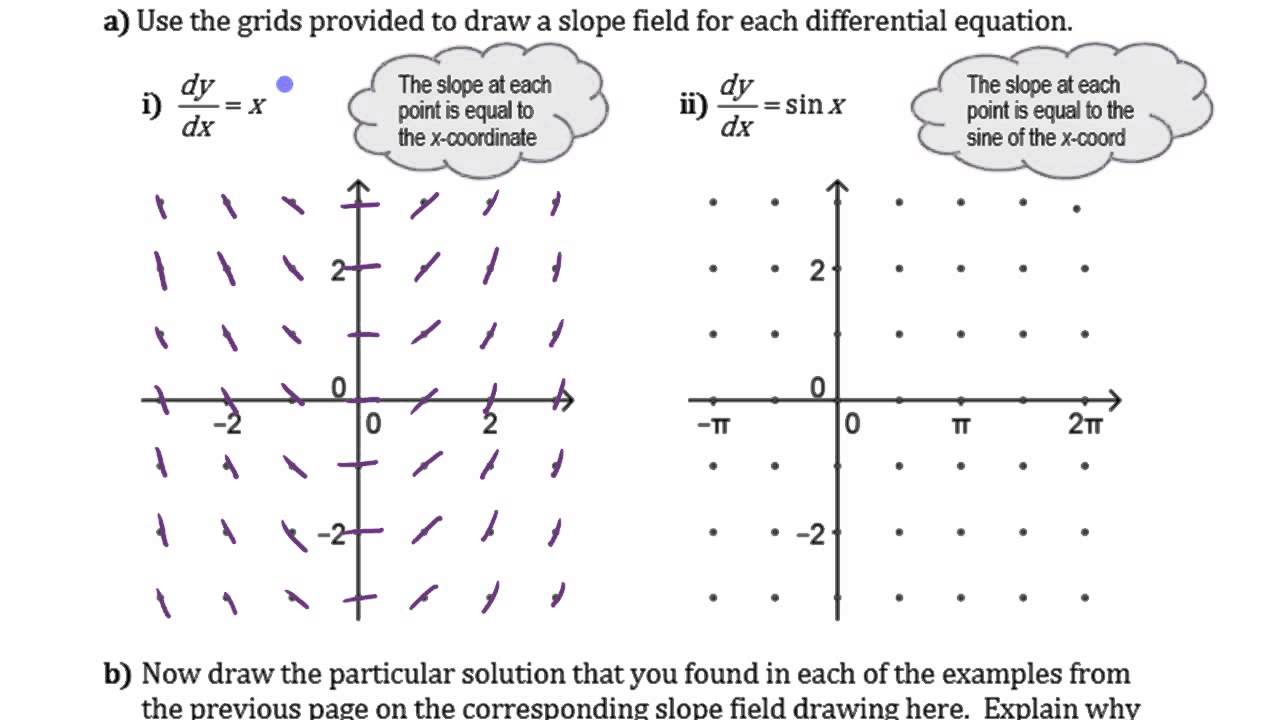
\includegraphics[width=0.5\linewidth]{images/Slope Fields.jpg}
        \caption{Slope Fields}
        \label{fig:slopeFields}
    \end{figure}
\end{itemize}

\end{document}